Using the data on $x_{3} = $holdover hours and $x_{4} = $COA hours from Table 5.8, construct
a prediction ellipse for a future observation $\textbf{x}^{\prime} = (x_{3}, x_{4})$. Remember, a prediction ellipse
should be calculated from a stable process Interpret the result.
\par
To see which values are stable, we compute the $T^{2}$ values as
\[
    T^{2}
    =
    \frac{n}{n+1}
    {(\textbf{x} - \bar{\textbf{x}})}^{\prime}
    \textbf{S}^{-1}
    (\textbf{x} - \bar{\textbf{x}})
\]
and checking which values are less than or equal to
\[
    \frac{(n-1)p}{n-p}
    F_{p,n-p}(\alpha)
    =
    \frac{(15)2}{14}
    F_{2,14}(0.05)
    =
    8.012
\]
This is the same as
\[
    {(\textbf{x} - \bar{\textbf{x}})}^{\prime}
    \textbf{S}^{-1}
    (\textbf{x} - \bar{\textbf{x}})
    \leq
    \frac{(n^{2} - 1)}{n(n - p)}
    F_{p,n-p}(\alpha)
\]
All of the values are less than the right-hand-side in the above, so we have a stable process. The future overtime ellipse for holdover and COA is below.

Half-lengths in the ellipse are computed as: $\sqrt{\lambda_{i}}\sqrt{\frac{(n+1)(n-1)p}{n(n-p)}F_{p, n-p}(\alpha)}$.

\begin{figure}[H]
    \centering
    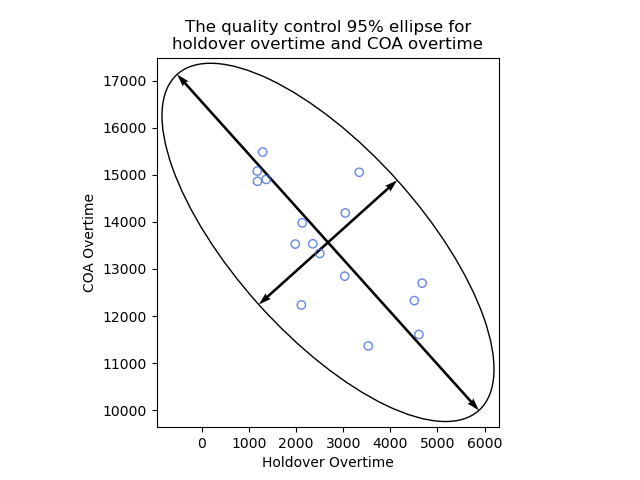
\includegraphics[scale=0.65]{./python/chapter-5/Question-5-27-Future-Ellipse.png}
\end{figure}

Any future observation falling within the ellipse is regarded as stable or in control.